\chapter{Introduction}
\section{General Introduction}
\textcolor{blue}{In questa sezione una breve panoramica su FEMOS su cosa \`e gi\`a stato implementato su cosa si vuole fare...}
\section{Case tests presentation}
\textcolor{blue}{In questa invece andiamo pi\`u nello specifico di questo lavoro presentando i casi test che verranno studiati...non penso sia il caso di trattare le equazioni qui dato che c'\`e tutto un capitolo sul modello e le equazioni usate}

\begin{figure}[!h]
\subfigure[]
{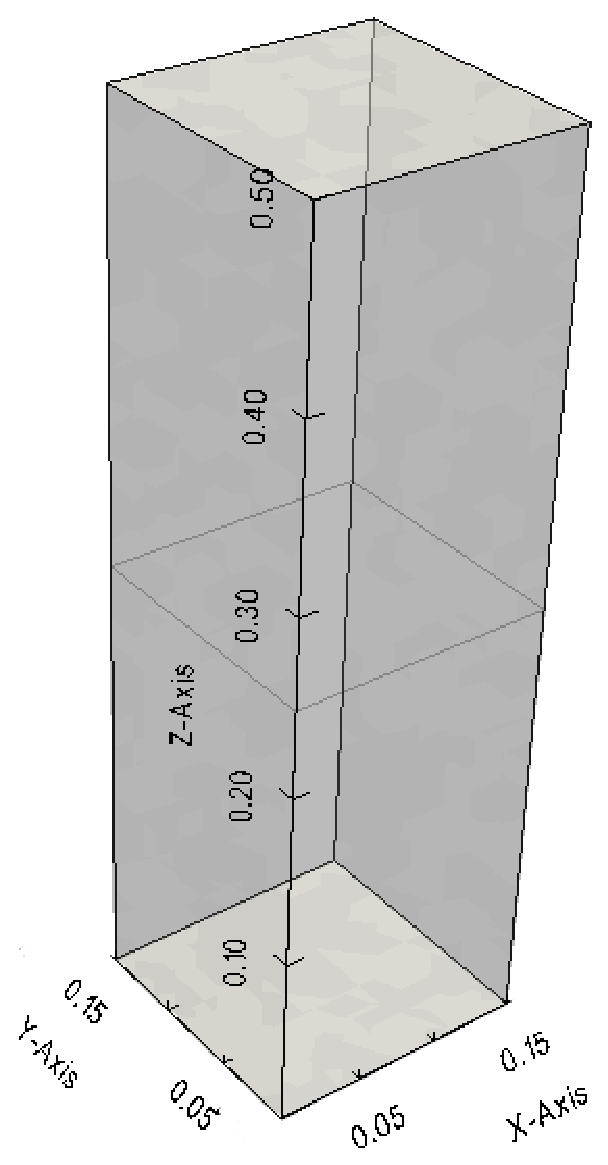
\includegraphics[height = 5.5cm,width = 3cm]{Casitest/DominioNP}}
\psp{10}
\subfigure[]
{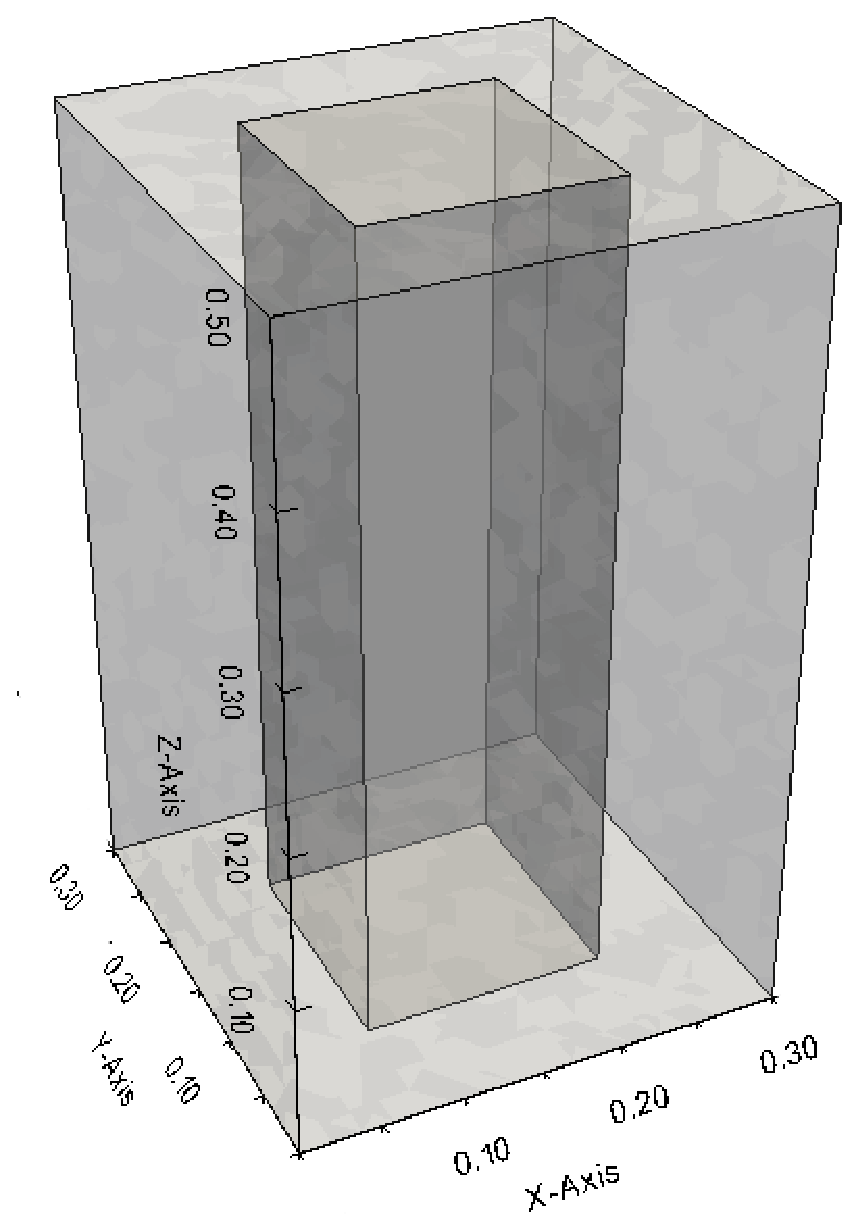
\includegraphics[height = 5.5cm,width = 3cm]{Casitest/DominioNPOX}}
\psp{10}
\subfigure[]
{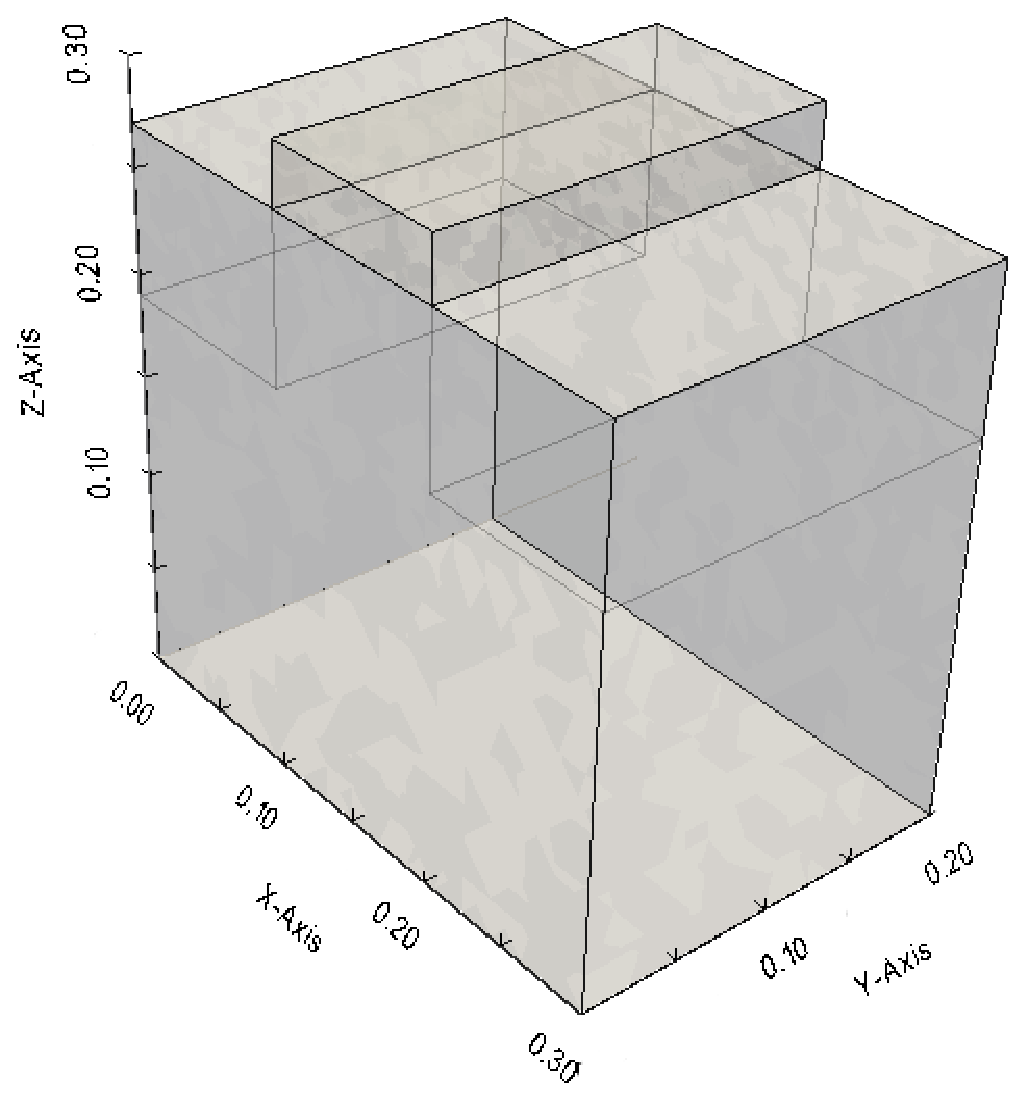
\includegraphics[height = 5.5cm,width = 4cm]{Casitest/DominioMOS}}
\end{figure}